% 2D Example Points
%
% File:         2d-points.tex
% Author:       Bob Walton (walton@acm.org)
% Date:      	Tue Dec 18 16:44:11 EST 2012
  
\documentclass{minimal}
\usepackage[paperheight=3in,paperwidth=6in,
            height=3in,hoffset=0.05in,
	    voffset=0.05in,left=0in,width=6in]{geometry}
\usepackage{color}
\usepackage[usenames]{xcolor}
\usepackage{tikz}
\begin{document}
\raggedright
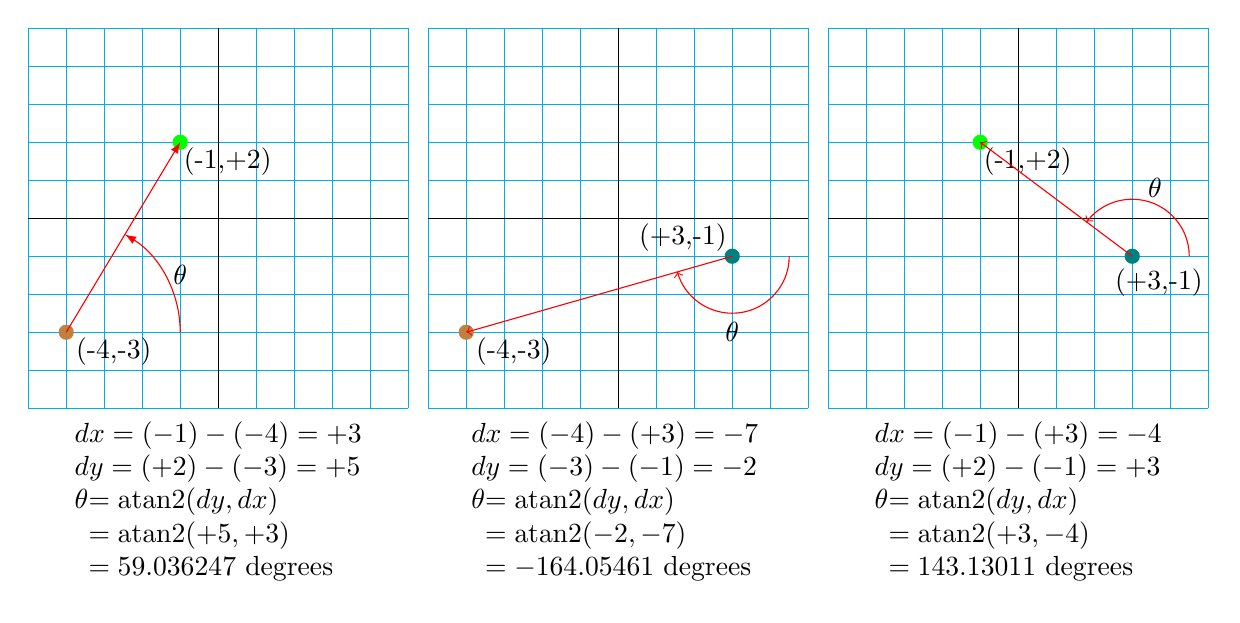
\begin{tikzpicture}[x=0.190in,y=0.190in]


\begin{scope}[xshift=0in,yshift=1in,>=latex]
    \draw[cyan] (-5,-5) grid[step=1] (5,5);
    \draw[black] (-5,0) -- (+5,0);
    \draw[black] (0,-5) -- (0,+5);
    \fill[green] (-1,+2) circle(0.2) + (+1.25,-0.5) node[black]{(-1,+2)};
    \fill[brown] (-4,-3) circle(0.2) + (+1.25,-0.5) node[black]{(-4,-3)};
    \draw[red,->] (-4,-3) -- (-1,+2);
    \draw[red,->] (-4,-3) + (+3,0) arc(0:59:3);
    \draw[black] (-1,-1.5) node{$\theta$};
\end{scope}

% Because coordinate (-5,-5) is used within the tikzpicture,
% it is the lower left.

\begin{scope}[xshift=0in,yshift=-0.8in]
    \draw (0,2) node{
	$\begin{array}{l}
	dx = (-1) - (-4) = +3 \\
	dy = (+2) - (-3) = +5 \\
	\theta \begin{array}[t]{@{}l}
	        = \mbox{atan2}(dy,dx) \\
		= \mbox{atan2}(+5,+3) \\
		= 59.036247~\mbox{degrees} \\
	        \end{array}
	\end{array}$
   };
\end{scope}

\begin{scope}[xshift=2in,yshift=1in]
    \draw[cyan] (-5,-5) grid[step=1] (5,5);
    \draw[black] (-5,0) -- (+5,0);
    \draw[black] (0,-5) -- (0,+5);
    \fill[teal] (+3,-1) circle(0.2) + (-1.3,+0.5) node[black]{(+3,-1)};
    \fill[brown] (-4,-3) circle(0.2) + (+1.25,-0.5) node[black]{(-4,-3)};
    \draw[red,->] (+3,-1) -- (-4,-3);
    \draw[red,->] (+3,-1) + (+1.5,0) arc(0:-164:1.5);
    \draw[black] (+3,-3) node{$\theta$};
\end{scope}

\begin{scope}[xshift=2in,yshift=-0.8in]
    \draw (0,2) node{
	$\begin{array}{l}
	dx = (-4) - (+3) = -7 \\
	dy = (-3) - (-1) = -2 \\
	\theta \begin{array}[t]{@{}l}
	        = \mbox{atan2}(dy,dx) \\
		= \mbox{atan2}(-2,-7) \\
		= -164.05461~\mbox{degrees} \\
	        \end{array}
	\end{array}$
   };
\end{scope}

\begin{scope}[xshift=4in,yshift=1in]
    \draw[cyan] (-5,-5) grid[step=1] (5,5);
    \draw[black] (-5,0) -- (+5,0);
    \draw[black] (0,-5) -- (0,+5);
    \fill[green] (-1,+2) circle(0.2) + (+1.25,-0.5) node[black]{(-1,+2)};
    \fill[teal] (+3,-1) circle(0.2) + (+0.7,-0.7) node[black]{(+3,-1)};
    \draw[red,->] (+3,-1) -- (-1,+2);
    \draw[red,->] (+3,-1) + (+1.5,0) arc(0:143:1.5);
    \draw[black] (+3.6,+0.8) node{$\theta$};
\end{scope}

\begin{scope}[xshift=4in,yshift=-0.8in]
    \draw (0,2) node{
	$\begin{array}{l}
	dx = (-1) - (+3) = -4 \\
	dy = (+2) - (-1) = +3 \\
	\theta \begin{array}[t]{@{}l}
	        = \mbox{atan2}(dy,dx) \\
		= \mbox{atan2}(+3,-4) \\
		= 143.13011~\mbox{degrees} \\
	        \end{array}
	\end{array}$
   };
\end{scope}
\end{tikzpicture}
\end{document}
